\begin{figure}[H]
	\centering
	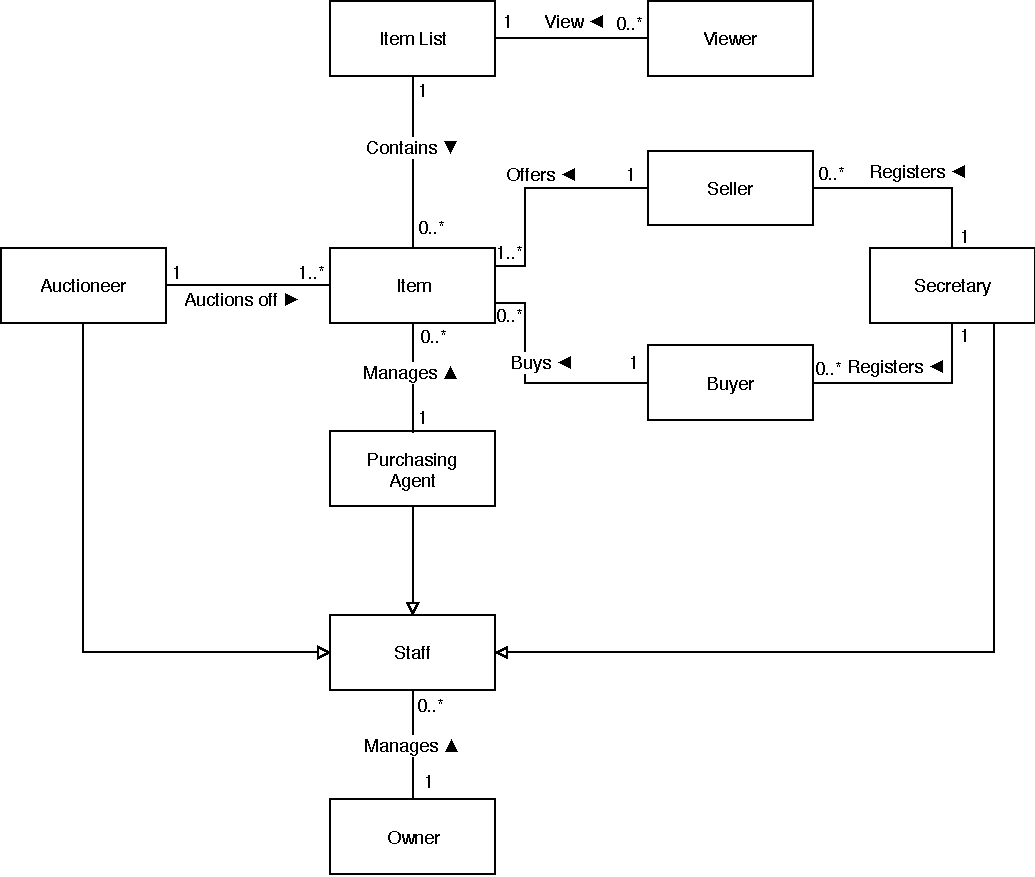
\includegraphics[scale=.9]{domainmodelUPD2.pdf}
\end{figure}
% arrows for domain models to copy: ► ◄ ▲ ▼

% Things to add:
% Search Request, Book (maybe multiple kinds and a catalogue, well see)
The domain model is a universal, graphical representation of the relevant concepts. It shows how all concepts relate to eachother. For example, you can see that items are `used' by a number of sources, such as buyers, sellers, the auctioneer and the purchasing agent. Items are also contained in an item list, which is just the collection of items. The item list can in turn be viewed by the public.\\
We also see that all staff is an instance of the staff class. Any staff is then managed by the owner of The AuctionHouse\textsuperscript{TM}. This does not only make sense for our customer, but also for a future implementation, even though that is not (yet) our concern.\\
We see that a number of parties can register something to the system. One is the secretary can add potential buyers and sellers to the system, granting them more permissions than the general public. Another is the purchasing agent, who can, after evaluation, add items to the system, making them available for viewing by the public.
There is no Auction concept in the domain model. The reason is that auctions are not going to be digitalized; they will still be physically held. Therefore, we do not concern ourselves with it when sketching the domain.